\documentclass{report}
\usepackage[utf8]{inputenc}
\usepackage{amsmath}
\usepackage{graphicx}

\title{Eksamensnoter - Fibonnaci Heaps}
\author{André Oskar Andersen (wpr684)}
\date{\today}

\begin{document}
\maketitle

\section*{19 Fibonnaci Heaps}
\begin{center}
    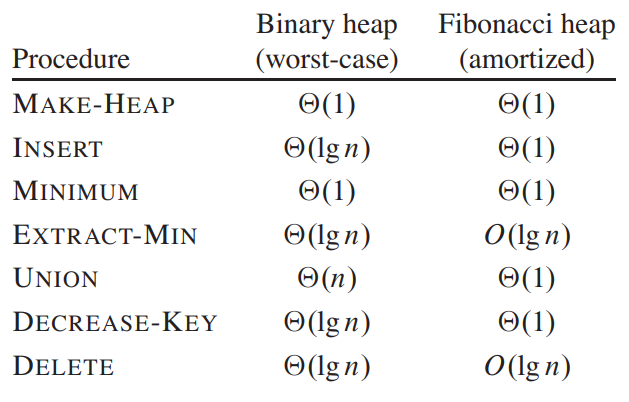
\includegraphics[width = 7 cm]{../entities/fib_heap_vs_bin_heap.png}
\end{center}
\begin{itemize}
    \item The Fibonacci heap data structure serves a dual purpose:
    \begin{enumerate}
        \item It supports a set of operations that constitutes what is known as a "mergeable heap"
        \item Several Fibonacci-heap operations run in constant amortized time, which makes this data structure well suited for applications that invoke these operations frequently
    \end{enumerate}
\end{itemize}
\textbf{Mergeable heaps}
\begin{itemize}
    \item A \textit{mergable heap} is any data structure that supports the following five operations, in which each element has a \textit{key}:
    \begin{itemize}
        \item \texttt{MAKE-HEAP()}: creates and returns anew heap containing no elements
        \item \texttt{INSERT(H, x)}: insert element $x$ into heap $H$ 
        \item \texttt{MINIMUM(H)}: returns a pointer to the element in heap $H$ whose key is minimum
        \item \texttt{EXTRACT-MIN(H)}: deletes the element from heap $H$ whose key is minimum, returning a pointer to the element
        \item \texttt{UNION($H_1$, $H_2$)}: creates and returns a new heap that contains all the elements of heaps $H_1$ and $H_2$.
    \end{itemize}
    \item In addition to the mergeable-heap operations above, Fibonacci heaps also support the following two operations:
    \begin{itemize}
        \item \texttt{DECREASE-KEY(H, x, k)}: assigns to element $x$ within heap $H$ the new key value $k$, which we assume to be no greater than its current key value
        \item \texttt{DELETE(H, x)}: deletes element $x$ from heap $H$
    \end{itemize}
\end{itemize}
\subsection*{19.1 Structure of Fibonacci heaps}
\begin{itemize}
    \item A \textit{Fibonacci heap} is a collection of rooted trees that are \textit{min-heap ordered}. That is, each tree obeys the \textit{min-heap property}: the key of a node is greater than or equal to the key of its parent.
    \item Each node $x$ contains a pointer $x.p$ to its parent and a pointer $x.child$ to any one of its children. The children of $x$ are linked together in a circular, doubly linked list, which we call the \textit{child list} of $x$. Each child $y$ in a child list has pointers $y.left$ and $y.right$ that point to $y$'s left and right siblings, respectively. If node $y$ is an only child, then $y.left = y.right = y$. Siblings may appear in a child list in any order.
    \item Each node has two other attributes:
    \begin{itemize}
        \item We store the number of children in the child list of node $x$ in $x.degree$
        \item The boolean-value attribute $x.mark$ indicates whether node $x$ has lost a child since the last time $x$was made the hcild of another node. Newly created nodes are unmarked, and a node $x$becomes unmarked whenever it is made the child of another node.
    \end{itemize}
    \item We access a given Fibonacci heap $H$ by a pointer $H.min$ to the root of a tree containing the minimum key; we call this node the \textit{minimum node} of the Fibonacci heap.
    \item The roots of all the trees in a Fibonacci heap are linked together using their \textit{left} and \textit{right} pointers into a circular, doubly linked list called the \textit{root list} of the Fibonacci heap. The pointer $H.min$thus points to the node in the root list whose key is minimum.
    \item We rely on one other attribute for a Fibonacci heap $H$: $H.n$, the number of nodes currntly in $H$
\end{itemize}
\textbf{Potential function}
\begin{itemize}
    \item For a given fibonacci heap $H$, we indicate by $t(H)$ the number of trees in the root list of $H$ and by $m(H)$ the number of marked nodes in $H$. We then define the potential $\Phi(H)$ of Fibonacci heap $H$ by
    $$\Phi(H) = t(H) + 2m(H)$$
\end{itemize}
\textbf{Maximum degree}
\begin{itemize}
    \item When only the mergeable-heap operations are supported, then the upper bound $D(n)$ on the maximum degree og any node in a $n$-node Fibonacci heap is; $D(n) \leq \left \lfloor{\lg n}\right \rfloor$. When we support \texttt{DECREASE-KEY} and \texttt{DELETE} as well; $D(n) = O(\lg n)$
\end{itemize}
\subsection*{19.2 Mergeable-heap operations}
\begin{itemize}
    \item No matter what the root list looks like before an \texttt{EXTRACT-MIN} operation, afterward each node in the root list has a degree that is unique within the root list, which leads to a root list of size at most $D(n) + 1$
\end{itemize}
\textbf{Creating a new Fibonacci heap}
\begin{itemize}
    \item To make an empty Fibonacci heap, the \texttt{MAKE-FIB-HEAP} procedure allocates and returns the Fibonacci heap object $H$, where $H.n = 0$ and $H.min = NIL$. Because $t(H) = 0$ and $m(H) = 0$, the potential of the empty Fibonacci heap is $\Phi(H) = 0$. The amortized cost of \texttt{MAKE-FIB-HEAP} is thus equal to its $O(1)$ actual cost
\end{itemize}
\textbf{Inserting a node}
\begin{itemize}
    \item To determien the amortized cost of \texttt{FIB-HEAP-INSERT}, let $H$ be the input Fibonacci heap and $H'$ be the resulting Fibonacci heap. Then, $t(H') = t(H) + 1$ and $m(H') = m(H)$, and the increase in potential is
    $$((t(H) + 1) + 2m(H)) - (t(H) + 2m(H)) = 1.$$
    Since the actual cost is $O(1)$, the amortized cost is $O(1) + 1 = O(1)$
\end{itemize}
\textbf{Finding the minimum node}
\begin{itemize}
    \item The minimum node of a Fibonacci heap \textit{H} is given by the pointer $H.min$, so we can find the minimum node in $O(1)$ actual time. Because the potential of $H$ does not change, the amortized cost of this operation is equal to its $O(1)$ acutal cost
\end{itemize}
\textbf{Uniting two Fibonacci heaps}
\begin{itemize}
    \item The change in potential is
    $$\Phi(H) - (\Phi(H_1) + \Phi(H_2))$$
    $$ = (t(H) + 2m(H)) - ((t(H_1) + 2m(H_1)) + (t(H_2) + 2m(H_2)) = 0$$
    because $t(H) = t(H_1) + t(H_2)$ and $m(H) = m(H_1) + m(H_2)$. The amortized cost of \texttt{FIB-HEAP-UNION} is therefore equal to its $O(1)$ actual cost
\end{itemize}
\textbf{Extracting the minimum node}
\begin{itemize}
    \item \texttt{FIB-HEAP-EXTRACT-MIN} works by first making a root out of each of the minimum node's children and removing the minimum node from the root list. It then consolidates the root list by linking roots of equal degree until at most one root remains of each degree
\end{itemize}

\end{document}